\documentclass[tikz]{standalone}
\usepackage{tikz}
\usepackage{siunitx}
\DeclareSIUnit\degF{\text{°}F}

\definecolor{codeblue}{RGB}{69, 161, 248}
\definecolor{codegray}{RGB}{40, 40, 40}
\usetikzlibrary{shapes,arrows}
\tikzstyle{decision} = [diamond, draw, fill=codegray, text=white,
    text width=4.5em, text badly centered, node distance=3cm, inner sep=0pt]
\tikzstyle{block} = [rectangle, draw, fill=codeblue,  text=white,
    text width=5em, text centered, rounded corners, minimum height=4em]
\tikzstyle{line} = [draw, -latex']


\begin{document}
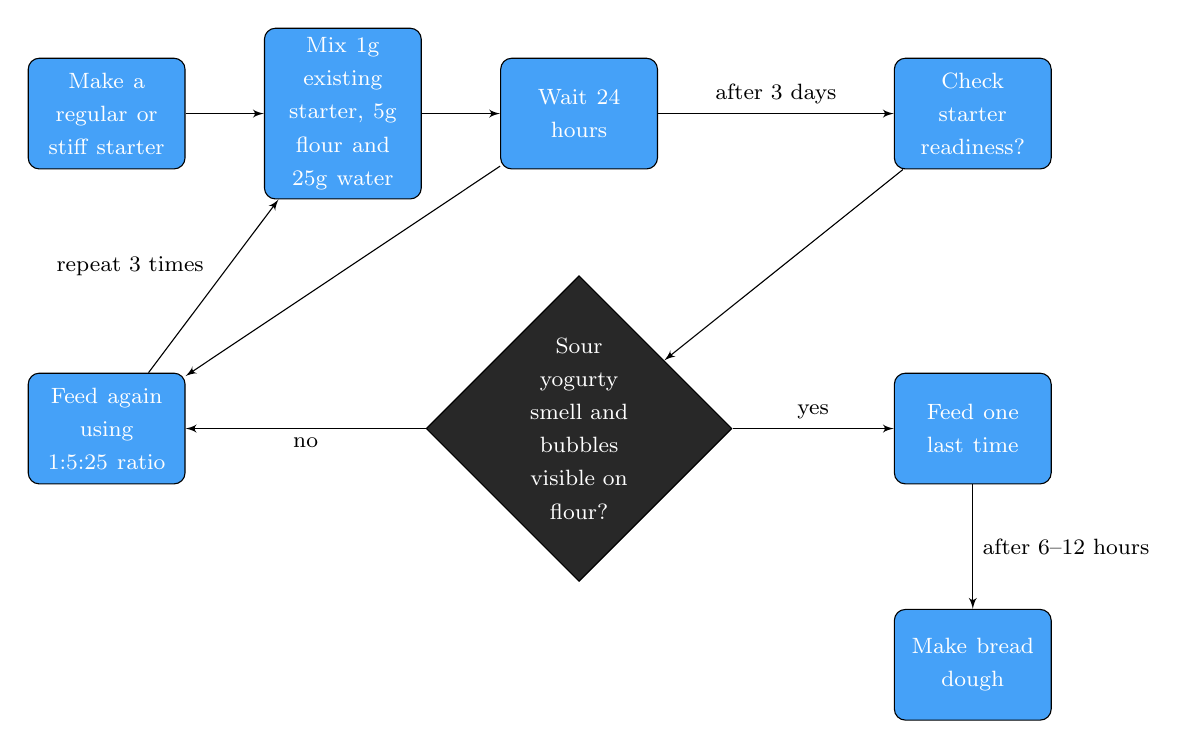
\begin{tikzpicture}[node distance = 3cm, auto]
  \node [block] (init) {\footnotesize Make a regular or stiff starter};
  \node [block, right of=init] (feed_new_ratio) {\footnotesize Mix 1g existing starter, 5g flour and 25g water};
  \node [block, right of=feed_new_ratio] (next_day) {\footnotesize Wait 24 hours};
  \node [block, below of=init, node distance=4cm] (feed_again) {\footnotesize Feed again using 1:5:25 ratio};
  \node [block, right of=next_day, node distance=5cm] (test) {\footnotesize Check starter readiness?};
  \node [decision, below of=next_day, node distance=4cm] (ready_signs) {\footnotesize Sour yogurty smell and bubbles visible on flour?};
  \node [block, below of=test, node distance=4cm] (last_feed) {\footnotesize Feed one last time};
  \node [block, below of=last_feed, node distance=3cm] (bread_dough) {\footnotesize Make bread dough};
  \path [line] (init) -- (feed_new_ratio);
  \path [line] (feed_new_ratio) -- (next_day);
  \path [line] (feed_again) -- node{\footnotesize repeat 3 times} (feed_new_ratio);
  \path [line] (next_day) -- node{\footnotesize after 3 days} (test);
  \path [line] (next_day) -- (feed_again);
  \path [line] (test) -- (ready_signs);
  \path [line] (ready_signs) -- node{\footnotesize no} (feed_again);
  \path [line] (ready_signs) -- node{\footnotesize yes} (last_feed);
  \path [line] (last_feed) -- node{\footnotesize after 6--12 hours} (bread_dough);
\end{tikzpicture}
\end{document}
